% Chapter Template

\chapter{Infraestructura} % Main chapter title

\label{Chapter1} % Change X to a consecutive number; for referencing this chapter elsewhere, use \ref{ChapterX}

En este capítulo se detallarán las herramientas base empleadas en la realización de este trabajo.

%----------------------------------------------------------------------------------------
%	SECTION Hardware
%----------------------------------------------------------------------------------------
\section{Hardware}

%-----------------------------------
%	SUBSECTION Sensor
%-----------------------------------
\subsection{Sensores RGBD}

Los sensores RGBD son sensores capaces de captar a parte de las componentes roja, verde y azul de la luz, información de profundidad (o "D" depth en inglés). 

En el 2010 Microsoft publicó el sensor Kinect para la consola de juegos Xbox 360 y Xbox One. Pronto se convirtió en uno de los dispositivos electrónicos más vendidos en todo el mundo después de su lanzamiento.

\begin{figure}[th]
\centering
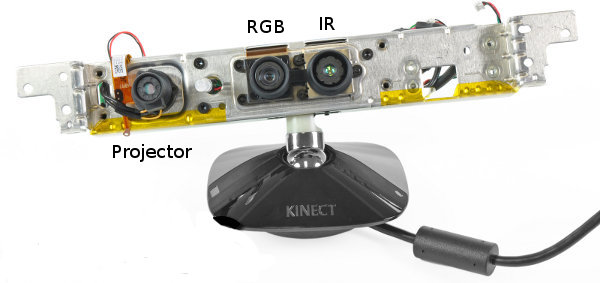
\includegraphics[scale=0.9]{Figures/ros_kinect.jpg}
\decoRule
\caption[Kinect sensor]{Sensor Microsoft Kinect}
\label{fig:Kinect}
\end{figure}

El sensor es capaz de combinar por cada pixel, la información de color con su correspondiente componente de profundidad. Esta tecnología fue desarrollada por la empresa israelí PrimeSense. El sensor Kinect dispone también de un micrófono multiarray con el cual puede predecir de dónde proviene el sonido.

Este sensor salió al mercado a un precio mucho más reducido que algunos que existían antes que él por lo que el interés por este tipo de sensores se disparó y comenzaron a aparecen en diferentes áreas de la tecnología, como interfaces naturales de usuario (en inglés natural user interface, NUI), reconstrucción y realidad virtual o cartografía 3D.

El sensor utilizado en este trabajo es el \textbf{Asus Xtion PRO LIVE} que dispone de la misma tecnología comercializado por Asus, que proporciona profundidad, color y audio (utilizando un micrófono multiarray como el sensor Kinect). \footnote{https://www.asus.com/3D-Sensor/Xtion\_PRO\_LIVE/}

\begin{figure}[th]
\centering
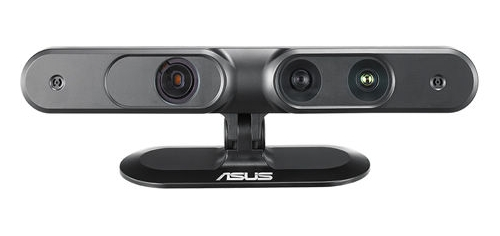
\includegraphics[scale=0.9]{Figures/xtion-pro-live.jpg}
\decoRule
\caption[Kinect sensor]{Asus Xtion PRO LIVE}
\label{fig:Kinect}
\end{figure}


\begin{table}
\caption{Especificaciones técnicas del Asus Xtion PRO LIVE}
\label{tab:xtion}
\centering
\begin{tabular}{ l | l }
\toprule
Campo de visión: & 58º H, 45º V, 70º D\\
\hline
Distancia de uso: & Entre 0.8m y 3.5m\\
\hline
Tamaño de la imagen de profundidad: & VGA (640x480) : 30 fps \\
				& QVGA (320x240): 60 fps\\
\hline
Resolución: & SXGA (1280*1024) \\
\bottomrule
\end{tabular}
\end{table}

Las especificaciones técnicas de este sensor se encuentran recogidas en la tabla ~\ref{tab:xtion}
%----------------------------------------------------------------------------------------
%	SECTION Software
%----------------------------------------------------------------------------------------
\section{Software}

%-----------------------------------
%	SUBSECTION JDeRobot
%-----------------------------------
\subsection{JDeRobot}

JDeRobot es un proyecto desarrollado por el grupo de robótica de la Universidad Rey Juan Carlos\footnote{http://jderobot.org}. Consiste en una plataforma de desarrollo de aplicaciones robóticas y de visión artificial. Está en su mayoría escrito en C++, donde disponen de una colección de componentes capaces de comunicarse a través de ICE middleware\footnote{https://zeroc.com/products/ice}, entre ellos se pueden encontrar herramientas, drivers, interfaces, librerías y tipos.

\subsubsection{Gazebo}

\subsubsection{Recorder y Replayer}

\subsubsection{CameraServer}

\subsubsection{RGBDViewer}

%\subsubsection{RGBPoint}

%Es una estructura de datos proporcionada por JDeRobot en la cual se pueden guardar puntos en tres dimensiones, y en la que es de mucha utilidad para crear nubes de puntos (o point cloud en inglés).

\subsubsection{OpenniServer}

OpenniServer es un driver de JDeRobot que es capaz de proporcionar a través de un sensor RGBD (Kinect o Xtion), imágenes de color, profundidad o nubes de puntos que son enviados a través de la interfaz ICE. Este driver se ha usado para este trabajo y es de donde se recogen tanto la imágen RGB como la de profundidad (DEPTH) para su posterior procesado.

\subsubsection{Progeo}

%-----------------------------------
%	SUBSECTION ICE
%-----------------------------------
\subsection{ICE}

%-----------------------------------
%	SUBSECTION PCL
%-----------------------------------
\subsection{Point Cloud Library (PCL)}

%-----------------------------------
%	SUBSECTION OpenCV
%-----------------------------------
\subsection{OpenCV}

OpenCV (Open Source Computer Vision Library) es una librería que proporciona estructuras de datos para guardar los diferentes tipos de imágenes (RGB, Depth), así como puntos o matrices con una gran cantidad de algoritmos para poder hacer operaciones con ellos.
